\chapter{情動ステアリングパイプライン}
\label{chap:development1_emo_steering}

本章では、コントラスティブ活性化加算（CAA）ベクトルが大規模言語モデル（LLM）の感情コンテキストにおいて構築可能であることを実証する。これらのベクトルは自然に\textbf{共有情動化成分}と\textbf{感情特異的残差成分}へと分解される。中心的な実証的知見は、信頼性の高い情動ステアリングには残差成分のみが必要であるという点である。

\section{章のロードマップ}
\label{sec:steering_roadmap_1}
本章はその主張に向けて構築される五つの段階を経て進行する。

\begin{enumerate}
  \item \textbf{前提条件}（\ref{sec:dataset_construction}節〜\ref{sec:layer_selection}節）：制御された感情書き換えデータセットを構築し、残差ストリーム活性化を抽出し、目標トランスフォーマー層を選択する。

  \item \textbf{CAAベクトルの構築}（\ref{sec:caa_construction}節）：感情条件付きおよび中性条件付きの隠れ状態の差分を取ることにより、各感情に対するコントラスティブベクトルを計算する。

  \item \textbf{観察}：得られたベクトルの感情間コサイン類似度は$0.91$〜$0.97$の範囲に集中しており、目標感情に関わらずベクトルが共有方向に支配されていることを示している。

  \item \textbf{分解}（\ref{sec:decomposition}節）：共有方向$\mathbf{g}$を射影除去することで感情特異的残差ベクトル$\hat{\mathbf{r}}_e$を得る。これにより二成分パラメータ化$\Delta_e = \alpha_G\,\mathbf{g}+\alpha_R\,\hat{\mathbf{r}}_e$が得られる。

  \item \textbf{ステアリング評価}（\ref{sec:steering_experiments}節）：推論時の実験により、残差成分のみで十分であることが示される。$\mathbf{g}$を含めること（$\alpha_G > 0$）はわずかに逆効果である。
\end{enumerate}

\section{データセット構築}\label{sec:dataset_construction}

感情が残差空間において構造化された幾何学として符号化されているかどうかを調査するため、共有ソース発話から制御された書き換えデータセットを構築した。主要データセットは、DailyDialog~\cite{li2017dailydialogmanuallylabelledmultiturn}とEmpatheticDialogues~\cite{rashkin2019empatheticopendomainconversationmodels}という二つの対話コーパスから派生した感情カテゴリ書き換えセットである。会話的発話は日常的な対人コンテキストに根ざしたコンパクトな感情信号を提供しつつ、命題的内容を制御された書き換えに十分なほど制約できることから、対話データを選択した。各ソース発話に対して、GPT-4.1-miniを使用してプルチックの八つの基本感情（\textit{joy}、\textit{trust}、\textit{fear}、\textit{surprise}、\textit{sadness}、\textit{disgust}、\textit{anger}、\textit{anticipation}）の書き換えを三段階の対応する強度レベル（低、中、高）で生成した。これによりソーステキスト一件あたり$8\times3 = 24$種類の情動的変形が得られる。構築全体を通じた中心的制約は意味保存であった。すなわち、基底となる状況と事実的内容を一定に保ちつつ、情動的フレーミングのみを体系的に変化させた。

\begin{table}[H]
\centering
\small
\begin{tabular}{p{0.12\linewidth} p{0.82\linewidth}}
\toprule
\textbf{感情} & \textbf{発話} \\
\midrule
\textbf{Base} & \textbf{I waited for hours and nobody came.} \\
Joy & Nobody came for hours, but I ended up enjoying the quiet time on my own. \\
Trust & Nobody came for hours, but I am sure they had a valid reason. \\
Fear & Nobody came for hours, and I started worrying that something might have gone wrong. \\
Surprise & Nobody came for hours, and honestly I did not expect that at all. \\
Sadness & For hours, nobody came. I guess that says enough. \\
Disgust & Nobody came for hours; that felt deeply inconsiderate. \\
Anger & Nobody came for hours, and I am really frustrated about wasting all that time. \\
Anticipation & Nobody came for hours, but I kept thinking they might still arrive any minute. \\
\bottomrule
\end{tabular}
\caption{対応する中強度における全八つのプルチック感情カテゴリの例示的書き換え。}
\label{tab:emotion_rewrite_example}
\end{table}

制御条件として、追加的な中性パラフレーズベースラインデータセットを構築した。各ソース発話は、情動的に中性でありながら意味的に等価な形式に書き換えられた。このベースラインは、目標とする感情的色付けのないコンテンツの参照表現を提供し、感情条件付き活性化と感情抑制活性化の間のコントラスティブ分析を可能にする。\par

\begin{table}[H]
\centering
\small
\begin{tabular}{p{0.22\linewidth} p{0.72\linewidth}}
\toprule
\textbf{フィールド} & \textbf{例} \\
\midrule
Base utterance & What a mess!  Sorry. I'll clean it up. \\
Neutral paraphrase & There is a mess. I will clean it up. \\
\bottomrule
\end{tabular}
\caption{中性パラフレーズ制御データセットからの例示的サンプル。}
\label{tab:neutral_rewrite_example}
\end{table}

これらのデータセットを組み合わせることで、感情信号を語彙・意味的内容から区別することが可能となり、後続のセクションで提示される復号可能性、幾何学、ステアリング分析の経験的基盤が提供される。この設計により、感情的変動が感情的な言葉間の表層的な語彙的差異を単に反映するのではなく、活性化空間において一貫したベクトルを形成するかどうかを問うことが可能になる。\par

感情書き換えデータセットはDailyDialogとEmpatheticDialoguesから抽出された$22{,}782$件のユニークなソース発話から構成され、合計$546{,}768$件の情動サンプル（$8$感情$\times$$3$強度レベル$\times$$22{,}782$件のベーステキスト）が得られる。中性パラフレーズ制御データセットには$22{,}782$件のサンプルが含まれ、ユニークなソース発話一件につき一件となっている。

\section{残差ストリーム抽出}
\label{sec:residual_extraction}

勾配更新なしで指示チューニング済み言語モデル（Llama-3.1-8B~\cite{meta2024llama318b}）から隠れ状態活性化を抽出する。順伝播と活性化抽出の実装にはHuggingFace Transformersライブラリ~\cite{wolf2020huggingfacestransformersstateoftheartnatural}を使用する。

条件間で入力が比較可能であることを保証するため、各サンプルは同一のベース発話から構築された共有指示プレフィックスを用いてフォーマットされる。継続テキストのみが変更され、感情書き換えまたは中性パラフレーズのいずれかを通じて行われる。具体的には、話者の気持ちに合わせた書き換えを要求するチャットテンプレートのユーザ指示を使用し、書き換えられた文をアシスタントの継続として追加する。このマッチングプロトコルはプロンプトレベルの分散を制御し、感情条件付き活性化と中性条件付き活性化の直接比較を可能にする。

\begin{table}[H]
\centering
\label{tab:activation_prompt}
\begin{tabular}{p{0.95\linewidth}}
\toprule
\textbf{テンプレートプロンプト} \\
\midrule
Please rewrite this so it aligns with my feelings more. \\
Start straight from the rewritten text without any preamble, and only provide \textbf{one} rewritten version. \\
Base: \texttt{\{base\_text\}} \\
\bottomrule
\end{tabular}
\caption{活性化抽出に使用するプロンプト形式。}
\end{table}

図~\ref{fig:residual_extraction}は順伝播中の残差ストリーム抽出を示している。ユーザトークンとアシスタントトークンの両方を含むプロンプトがトランスフォーマースタックを通過し、選択された層で隠れ状態が記録される。各トランスフォーマーブロックはアテンションとMLP副層を通じて残差ストリームを更新し、層ごとの活性化$h^\ell \in \mathbb{R}^{T \times d_\text{model}}$を生成する。ここで$T$はトークン数、$d_\text{model}$は隠れ次元である。

\begin{figure}[H]
    \centering
    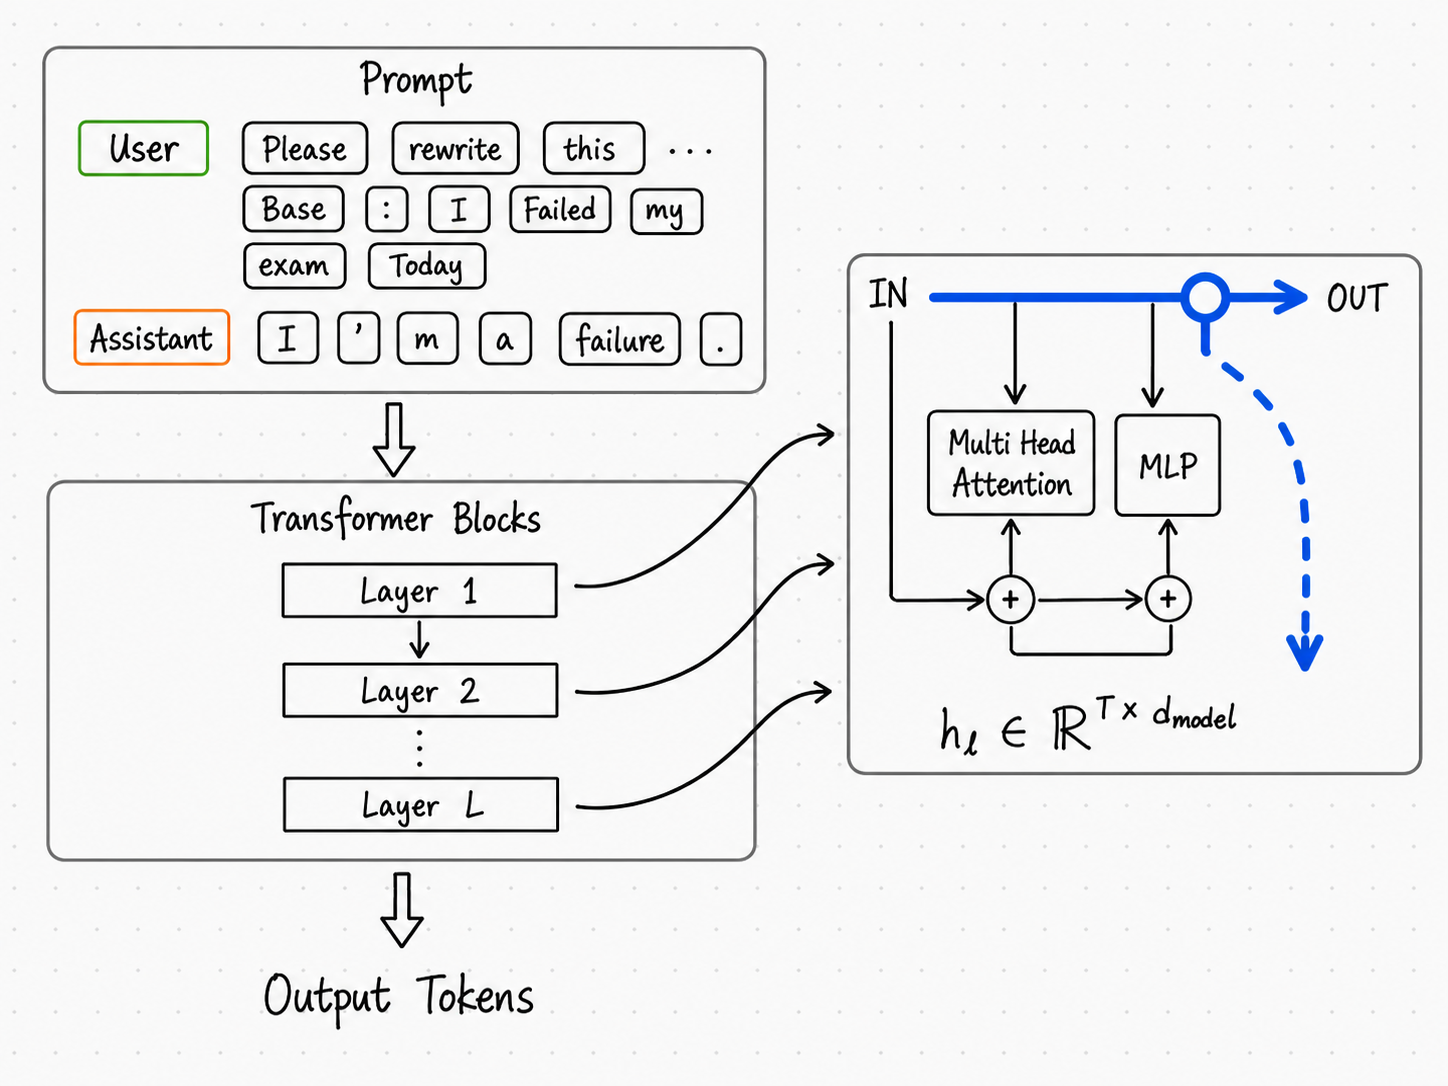
\includegraphics[width=0.6\linewidth]{figures/residual_extraction.png}
    \caption{順伝播中の残差ストリーム抽出の概略図。トークン化プロセスは明確化のために簡略化されている。実際には、入力はサブワード単位にトークン化される（例：「please」は「ple」と「ase」にトークン化される場合がある）。}
    \label{fig:residual_extraction}
\end{figure}

各目標層$l$について、最終トークンの隠れ状態を層の出力から取得する。すなわち、
\[
\mathbf{h}_{l}=\texttt{hidden\_states}[l+1][:,-1,:]
\]
トークン化は左パディングを使用するため、インデックス$-1$は各シーケンスの最後の実際のトークンに一貫して対応する。最終トークン表現は書き換えられた発話全体を処理した後のモデルの状態を捉え、継続によって表現される情動的フレーミングのコンパクトな要約となる。活性化は層$\{8,10,13,16,19,22\}$からサンプリングされ、全入力に対して多層表現が生成される。

まとめると、感情強度抽出パイプラインは5次元テンソルを生成する：
\[
\mathbf{H}^{\text{emo}} \in \mathbb{R}^{N \times E \times I \times L \times D},
\]
ここで$N$はソーステキスト数、$E=8$は感情書き換え数、$I=3$は強度レベル数、$L$はサンプリング層数、$D=4096$は隠れ次元である。中性ベースラインパイプラインは以下を生成する：
\[
\mathbf{H}^{\text{neu}} \in \mathbb{R}^{N \times L \times D}.
\]
ソースIDをソートして両テンソルをインデックスで整合させ、直接減算を可能にする：
\[
\Delta\mathbf{H}_{n,e,i,l,:}=\mathbf{H}^{\text{emo}}_{n,e,i,l,:}-\mathbf{H}^{\text{neu}}_{n,l,:},
\]
これによりベース意味的内容を制御しつつ情動的シフトを分離する。

\section{層選択と診断}
\label{sec:layer_selection}

全てのトランスフォーマー層が情動分析に等しく有用な表現を提供するわけではない。感情関連の構造は複数の深さで存在する可能性があるが、異なる層は表現の異なる特性を優先する場合がある。ロードマップ（\ref{sec:steering_roadmap_1}節）で説明したように、層選択段階の目的は前言語的感情が最もよく抽象化される層を特定することである。例えば、ある層は強い感情カテゴリ分離可能性を提供し、別の層はコンパクトな低次元幾何学をより良く保存するかもしれない。候補層を評価するために三つの診断指標を定義する：

\begin{enumerate}
  \item \textbf{バランス精度}：この指標は、その層が感情カテゴリ情報を保持するかどうかを測定する。PCAによって4次元部分空間に射影された残差ベクトルから感情カテゴリを予測するロジスティック回帰モデルを訓練する。値が高いほど、残差空間が人間が命名した感情ラベルへ線形写像できるように構成されていることを示す。
  \item \textbf{幾何学的コンパクト性}：この指標は感情情報が低次元部分空間に集中しているかどうかを測定する。残差空間における感情重心の説明分散比（EVR）を計算する。値が高いほど、少数のPCA/SVD成分が全残差ベクトルセットの分散の大部分を説明できることを示す。
  \item \textbf{段階的感情感度}：この指標は、その層の表現が感情カテゴリを単に分離するのではなく、感情強度を連続変数として符号化するかどうかを定量化する。各感情ラベルについてPCAを実行し、全サンプルを最初の主成分（PC1）、すなわち感情内分散が最大の軸に射影する。これらのPC1スコアと強度ラベル（低、中、高）の間のスピアマン相関は、感情内の支配的な方向が情動強度と一致するかどうかを示す。八つの感情にわたるこの相関の平均を報告する。
\end{enumerate}

\begin{table}[H]
\centering
\small
\begin{tabular}{lccc}
\toprule
\textbf{層} &
  \textbf{バランス精度} &
  \textbf{EVR\textsubscript{4}} &
  \textbf{段階的感情感度} \\
  & \textit{（4次元部分空間）} & & \\
\midrule
  8  & 0.6914 & 0.8834 & 0.1312 \\
  10 & 0.6751 & 0.8876 & 0.0998 \\
  13 \textbf{*} & \textbf{0.7033} & 0.8920 & \textbf{0.1336} \\
  16 & 0.6704 & \textbf{0.8958} & 0.1297 \\
  19 & 0.6198 & 0.8902 & 0.1142 \\
  22 & 0.6142 & 0.8928 & 0.1022 \\
\bottomrule
\end{tabular}
\caption{候補層の層ごとの診断サマリー。感情カテゴリプローブのバランス精度（4次元部分空間）、重心コンパクト性（EVR\textsubscript{4}）、および平均局所強度ベクトル相関。太字は各列の最良値を示し、アスタリスクは選択された報告層を示す。}
\label{tab:layer_diagnostics}
\end{table}

これらの診断に基づき、層13が主要分析の一次層として選択された。全ての指標で全体的に最良というわけではないが、上記三つの基準の間で最も説得力のあるトレードオフを提供する。

\begin{figure}[H]
    \centering
    
\includegraphics[width=0.8\linewidth]{figures/layer_diagnostics_lineplot.pdf}
    \caption{候補層にわたる層診断の可視化。}
    \label{fig:layer_diagnostics}
\end{figure}

第一に、\textbf{layer 13 achieves the highest balanced accuracy of all candidate layers}。バランス精度は残差部分空間において$0.7033$に達し、層8の$0.6914$、層10の$0.6751$、層16の$0.6704$と比較される。これは層13における情動表現が、少数の次元への圧縮後でさえ、人間が命名した感情カテゴリへ最も容易に写像できることを示唆する。これは必ずしもモデルが感情を離散的な記号ラベルとして表現していることを意味しない。むしろ、この層における連続的な情動幾何学が、単純な線形分類器が人間の感情カテゴリを回復できるように構成されていることを示している。\par

第二に、\textbf{layer 13 preserves a highly compact, low-dimensional geometry}。重心レベルの$\mathrm{EVR}_{4}$は$0.8920$であり、上位四つの主成分が感情重心間の分散の$89.2\%$を説明する。層16がわずかに高い$\mathrm{EVR}_{4}$（$0.8958$）を達成するが、差は小さい。層13における強いカテゴリ復号可能性は、低次元情動構造のコストとしてもたらされているわけではないようだ。層13はコンパクトかつ解釈可能な幾何学を保持している。\par

第三に、\textbf{layer 13 shows the highest graded affect sensitivity of all tested layers}。平均強度ベクトル相関は層13で$0.1336$であり、層8の$0.1312$、層10の$0.0998$、層16の$0.1297$と比較される。絶対値が控えめであることを考慮し、各感情の局所PC1を純粋な強度軸として解釈することはしない。むしろ、この指標は感情内の支配的な変動が情動強度との単調関係を保持するかどうかを示す。層13での高い値は、隣接する層よりもわずかに多くの段階的情動情報を保持していることを示唆する。\par

これらの診断を総合すると、層13は前言語的情動構造の有用な抽象化点に近いことが示唆される。初期の層（8および10）は相当量の情動情報を保持しているが、カテゴリ回復可能性と段階的感度は弱いか不安定である。後期の層（例：層16）はわずかにコンパクトな幾何学を持つが感情カテゴリのバランス精度が低く、後期の表現が言語化によってますます形成されていることを示唆する。層13は最良のトレードオフを提供する。すなわち、幾何学的分析を支援するのに十分な低次元性、人間の感情ラベルを回復するための線形組織性、そして段階的情動変動を保持するのに十分な感度を持つ。\par

したがって、後続の分析では層13を主要報告層として使用する。情動構造が存在する唯一の層として扱うわけではない。隣接する層は同様の傾向を示しており、情動幾何学が単一のトランスフォーマーブロックに局在するのではなく、複数の中間層にわたって分散していることを示している。層13は本研究の最も適切な操作層として理解されるべきである。すなわち、感情が明示的な言語ラベルに収縮される前に、感情のモデリングに表現が最も有用である層である。\par

\section{CAAベクトルの構築}
\label{sec:caa_construction}

\begin{figure}[H]
    \centering
    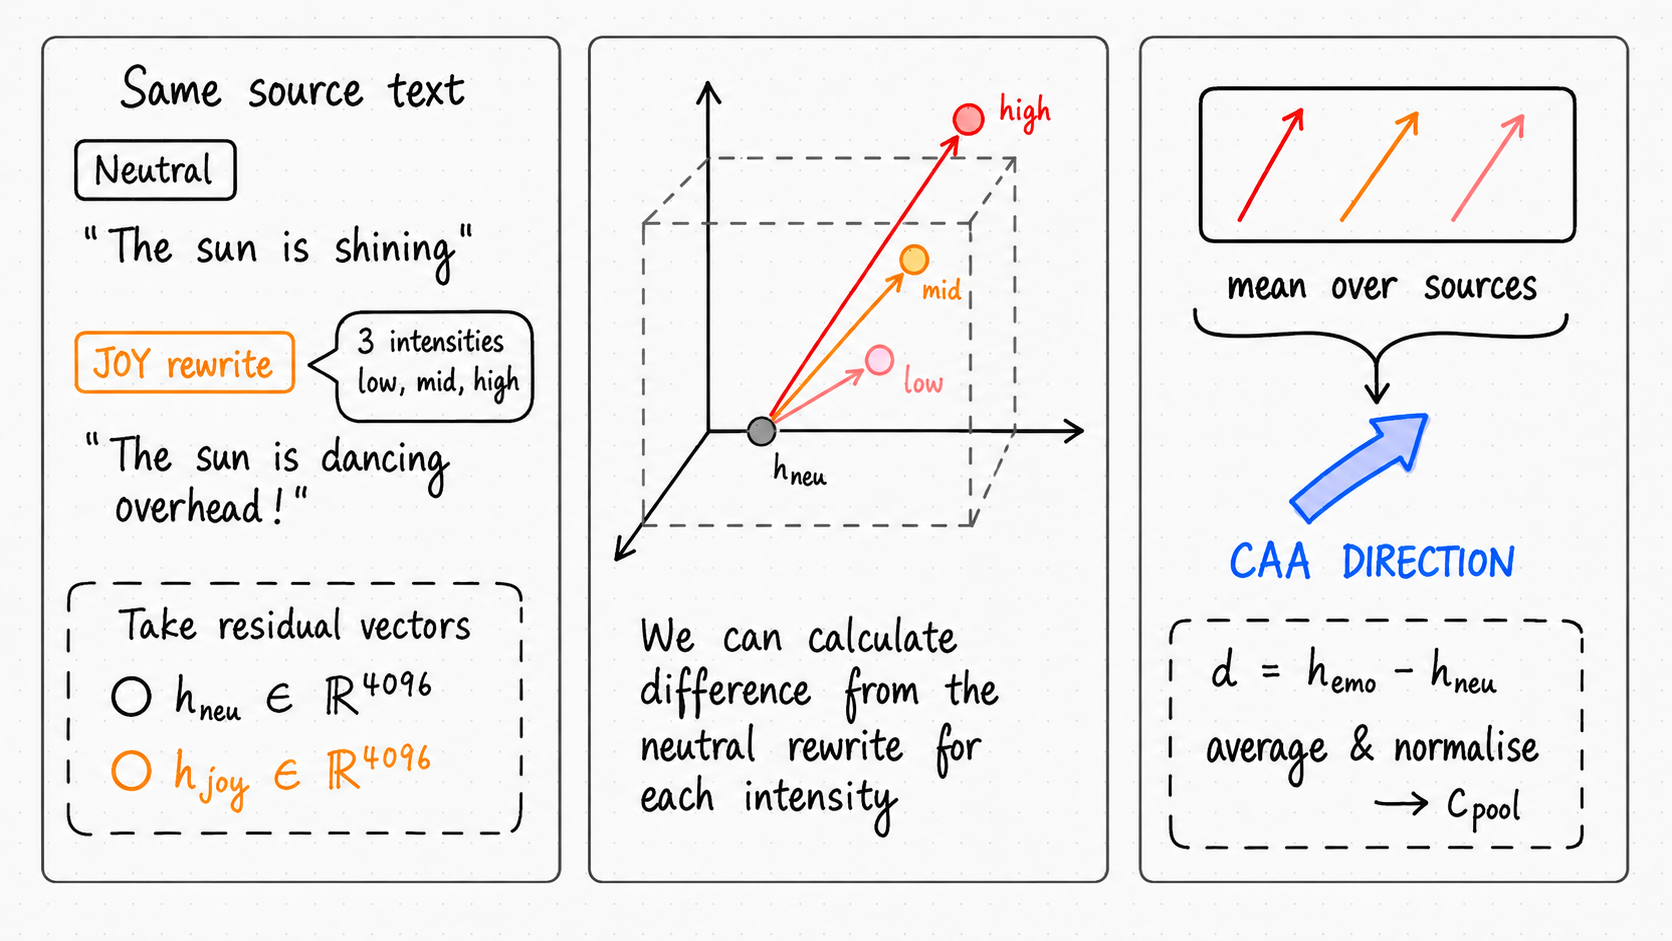
\includegraphics[width=0.6\linewidth]{figures/caa_construction.png}
    \caption{CAAベクトル構築の概略図。}
    \label{fig:caa_construction}
\end{figure}

コントラスティブ残差差分を制御可能なステアリング信号に変換するため、感情条件付きおよび中性条件付き活性化からCAA（コントラスティブ活性化加算）ベクトルを導出する。各ソース発話$n$、感情$e$、強度レベル$i$、層$l=13$について、まず以下を定義する：
\[
\Delta_{n,e,i,l}=\mathbf{h}^{\mathrm{emo}}_{n,e,i,l}-\mathbf{h}^{\mathrm{neu}}_{n,l}.
\]
次にソースにわたって平均を取り、単位長に正規化する：
\[
\bar{\Delta}_{e,i,l}=\frac{1}{N}\sum_{n=1}^{N}\Delta_{n,e,i,l},
\qquad
\mathbf{c}_{e,i,l}=\frac{\bar{\Delta}_{e,i,l}}{\lVert\bar{\Delta}_{e,i,l}\rVert_2}.
\]
ベクトル$\mathbf{c}_{e,i,l}$は強度特異的CAAベクトルである。

ステアリング段階は主として感情カテゴリを目標とし、強度を二次的な変調として扱うため、強度にわたって平均を取り再正規化することで\textbf{プールド感情ベクトル}$\mathbf{c}^{\mathrm{pool}}_{e,l}$も構築する：
\[
\mathbf{c}^{\mathrm{pool}}_{e,l}
=
\frac{\frac{1}{I}\sum_{i=1}^{I}\bar{\Delta}_{e,i,l}}
{\left\lVert\frac{1}{I}\sum_{i=1}^{I}\bar{\Delta}_{e,i,l}\right\rVert_2}.
\]

主要なステアリング分析では、これらのプールドユニットベクトルが主要な候補ステアリングベクトルとして使用される。\par

図~\ref{fig:caa_construction}は構築プロセスを示している。各感情と強度について、ソースにわたる平均コントラスティブシフトを計算し、正規化してユニットベクトルを得る。プールドベクトルは強度特異的ベクトルを平均し再正規化することで得られる。これにより、ステアリング介入のための感情特異的CAAベクトルのセットが得られる。\par

まず構築が安定していることを確認する。層13において、ソースごとのコントラスティブシフト$\Delta_{n,e} = h^\text{emo}_{n,e} - h^\text{neu}_n$とグローバルCAAベクトル$\mathbf{c}^\text{pool}_{e,13}$の間の平均コサイン類似度は$0.8536$から$0.8570$（標準偏差$\approx 0.054$）の範囲にある。これにより、平均ベクトルが少数の極端なサンプルによる人工物ではなく代表的であることが確認される。\par

しかし、感情カテゴリにわたる方向を調べると、驚くべきパターンが明らかになる。データセットに固有のソースペアリング構造を保持するため、感情間の類似度をソーステキストごとに計算し平均する。各ペア$(e_1, e_2)$について、$\frac{1}{N}\sum_n \cos(\hat{\Delta}_{n,e_1},\,\hat{\Delta}_{n,e_2})$を報告する。ここで$\hat{\Delta}_{n,e}$は強度にわたってプールされたソースごとの単位正規化シフトである。対角要素は感情内の強度一貫性を示す。すなわち、同一感情の低・中・高強度シフトにわたるソースごとの平均コサインである。結果の行列を図~\ref{fig:caa_paired_inter_emotion_cosine_heatmap_L13}に示す。\par

\begin{figure}[H]
  \centering
  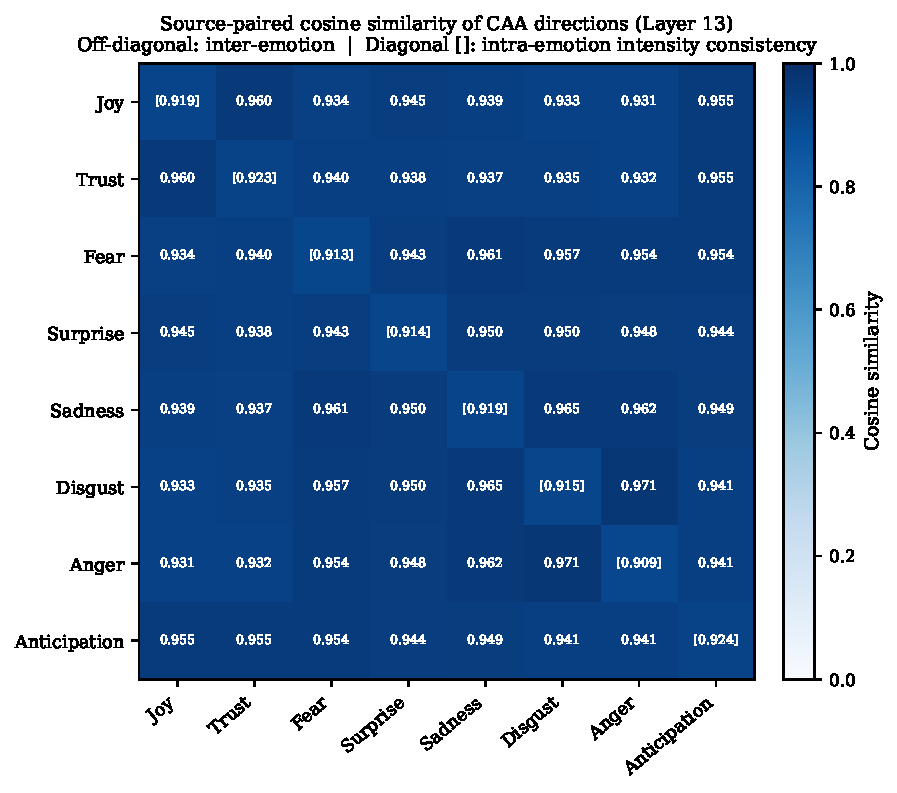
\includegraphics[width=0.75\linewidth]{figures/caa_paired_inter_emotion_cosine_heatmap_L13.pdf}
  \caption{層13におけるCAAディレクションのソースペアコサイン類似度。非対角：感情ペア間のソースごとの平均コサイン。対角\texttt{[\,]}：感情内強度一貫性（低・中・高強度ペアにわたるソースごとの平均コサイン）。カラースケールは$[0, 1]$に及び、全エントリが$0.90$を超えている。}
  \label{fig:caa_paired_inter_emotion_cosine_heatmap_L13}
\end{figure}

全ての値は$0.91$〜$0.97$の範囲にある。さらに際立つことに、\textit{disgust}--\textit{anger}（$0.971$）や\textit{sadness}--\textit{disgust}（$0.965$）などいくつかの感情ペアでは、感情間類似度が対角上の感情内強度一貫性（$0.91$〜$0.92$）を超えている。同一ソーステキストに対して、\textit{disgust}への方向は低強度の\textit{disgust}シフトが高強度の\textit{disgust}シフトに類似するよりも、\textit{anger}への方向に類似している。\par

この均一性は、各CAAベクトルが主として感情特異的情報を符号化している場合には予期されないものである。代わりに、\textbf{全てのベクトルが共有情動化成分に支配されている}ことが示唆される。この共通軸は目標感情に関わらず活性化される。\par

モデルは二つの段階で表現をシフトさせるように見える。まず中性文から汎用的な感情文へと移動する。次にその共有感情コンテキストから特定の情動カテゴリへと移動する。生のCAAベクトルは両段階を混同しており、感情特異的信号への直接アクセスを困難にする。この観察が、次節で導入される明示的な分解を動機付ける。\par

\section{分解}
\label{sec:decomposition}

層13のプールドCAAベクトルは感情カテゴリにわたって高度に整合しており、各ベクトルが汎用的な情動化に対応する大きな共有成分を含んでいることを示唆する。この共通シフトを感情特異的アイデンティティから分離するため、共有ベクトル$\mathbf{g}$を感情特異的プールドCAAベクトルにわたる正規化平均として定義する：
\[
\mathbf{g}=
\frac{\frac{1}{|E|}\sum_{e\in E}\mathbf{c}^{\mathrm{pool}}_{e,13}}
{\left\lVert\frac{1}{|E|}\sum_{e\in E}\mathbf{c}^{\mathrm{pool}}_{e,13}\right\rVert_2}.
\]
次に直交射影によって各プールドベクトルからこの共有成分を除去する：
\[
\mathbf{r}_e=\mathbf{c}^{\mathrm{pool}}_{e,13}-\left((\mathbf{c}^{\mathrm{pool}}_{e,13})^\top \mathbf{g}\right)\mathbf{g}.
\]
ステアリングには単位正規化された残差を使用する：
\[
\hat{\mathbf{r}}_e=\frac{\mathbf{r}_e}{\lVert\mathbf{r}_e\rVert_2},
\]
そして介入を以下のように構築する：
\[
\Delta_e(\alpha_G,\alpha_R)=\alpha_G\mathbf{g}+\alpha_R\hat{\mathbf{r}}_e.
\]

本章では、この分解を制御可能なステアリングのための操作的パラメータ化として扱う。$\mathbf{g}$は全体的な情動化強度を制御し、$\hat{\mathbf{r}}_e$は感情特異的方向性を制御する。
CAAの基礎仮定は、行動的特徴が残差ストリームの方向として近似できるというものである。分解はこの仮定に基づき、そのような方向に沿ってベクトルを加算することが対応する行動を因果的に変調するという前提に立つ。感情特異的CAAベクトルが強く整合している場合、その共有方向は全カテゴリにわたる感情応答に共通する成分を自然に推定する。\par

平均方向$\mathbf{g}$は感情カテゴリにわたって一貫して存在する成分を捉える。カテゴリ特異的成分は$e$によって変化することが期待されるため、感情にわたる平均化により、共通方向を保持しつつアイデンティティ関連の特異成分が低減される。したがって、$\mathbf{g}$を汎用的な情動化の推定値として解釈する。すなわち、特定の感情ラベルとは無関係に出力の全体的な感情的性格を高める方向である。\par

残差ベクトル\(\mathbf{r}_e\)は、\(\mathbf{c}^{\mathrm{pool}}_{e,13}\)を\(\mathbf{g}\)へ直交射影したものを減算することで得られる。これにより、共有情動化方向によって説明される感情特異的CAAベクトルの部分が除去される。その結果、\(\mathbf{r}_e\)は\(\mathbf{r}_e^\top \mathbf{g}=0\)を満たす。線形残差ストリーム近似の一次において、\(\hat{\mathbf{r}}_e\)に沿った変化は汎用的な情動化座標を直接変更しない。残差は残りのカテゴリ特異的変動を分離する。すなわち、共有感情シフトから特定の感情を区別するベクトルの部分である。\par

\(\mathbf{r}_e\)をさらに単位正規化することで方向と介入強度が分離される。残差ノルムはデータセットサイズ、カテゴリ内分散、プーリングの選択、または特定の感情が層13でどれだけ強く表現されているかに依存する場合がある。正規化された残差を使用することで、係数\(\alpha_R\)は感情間で比較可能な解釈を持つ。すなわち、残差ベクトルの大きさにおける恣意的な差異を継承することなく、活性化をカテゴリ特異的残差方向においてどれだけ移動させるかを制御する。\par

最終的な介入
\[
\Delta_e(\alpha_G,\alpha_R)=\alpha_G\mathbf{g}+\alpha_R\hat{\mathbf{r}}_e
\]
は二つの独立に解釈可能なステアリング制御を提供する。\(\alpha_G\)は共有情動化成分を変調し、\(\alpha_R\)は感情特異的残差成分を変調する。この分離により、感情強度と感情アイデンティティを独立して制御できるかどうかを検証することが可能である。\(\alpha_G\)を増加させると主として情動化の度合いが増加し、\(\alpha_R\)を増加させると主として目標感情の認識可能性が増加するはずである。\par

この手順は感情表現の単一の正確な分解を回復するものとして理解されるべきではない。むしろ、プールド感情CAAベクトル間で観察された高度な整合性によって駆動される、意図的に制約された線形分解である。得られた二パラメータ介入は、汎用的な情動化と感情特異的アイデンティティの間に意図した行動的解離を示すかどうかを実証的に評価される。\par

\begin{figure}[H]
    \centering
    
\includegraphics[width=0.8\linewidth]{figures/g_residualisation.png}
    \caption{感情CAAベクトルを共有情動化成分$g$と感情特異的残差成分$\hat{r}_e$への操作的分解。左パネルは三つの例示的感情（\textit{joy}、\textit{disgust}、\textit{sadness}）の元のCAAベクトルを示す。右パネルは共有成分$g$を除去した後の同じベクトルを示し、各感情に特有の残差ベクトル$\hat{r}_e$を明らかにしている。}
    \label{fig:g_residualisation}
\end{figure}

\section{分解の妥当性}
\label{sec:decomposition_validity}

\ref{sec:decomposition}節で導入された分解は幾何学的仮定に基づいている。すなわち、$\mathbf{g}$が全感情CAAベクトルに共通するものを捉え、$\hat{\mathbf{r}}_e$が感情識別情報を保持するという仮定である。本節では三つの独立した分析でその仮定を検証する。第一の分析は$\mathbf{g}$を射影除去することで感情間整合性が低下するかどうかを調べ、共有成分が\ref{sec:caa_construction}節で観察された高いコサイン類似度の原因であったことを確認する。第二の分析は$\hat{\mathbf{r}}_e$が感情を分類するのに十分かどうかを検証し、残差がカテゴリ情報を破棄するのではなく保持することを確認する。第三の分析は、残差化前には不明瞭であったプルチックの円形隣接構造~\cite{plutchik1980emotion}が、$\mathbf{g}$を除去した後に可視化されるかどうかを調べる。\par

\subsection{ソースペアコサイン類似度}

\ref{sec:caa_construction}節と同じソースペアプロトコルを使用して感情間コサイン類似度を計算する。各ペア$(e_1, e_2)$と各ソース$n$について、$\hat{\Delta}_{n,e_1}$と$\hat{\Delta}_{n,e_2}$の間のコサインを測定し、ソースにわたって平均する。対角エントリは感情内強度一貫性を測定する。この行列を二回計算する。一回はプールドCAAベクトル$\mathbf{c}^{\mathrm{pool}}_{e}$（残差化前）に対して、もう一回は単位正規化残差$\hat{\mathbf{r}}_e$（残差化後）に対してである。\par

図~\ref{fig:caa_decomposition_cosine_before_after_L13}に結果のヒートマップを示す。残差化前、全非対角エントリは$0.93$〜$0.97$の範囲にあり、平均は$0.947$である。残差化後、同じエントリは$0.73$〜$0.89$に低下し、平均は$0.794$である。$\Delta = -0.153$の減少により、$\mathbf{g}$が感情間整合性の主要な原因であったことが実証される。これを除去することで、八つの感情方向は互いに実質的により独立したものになる。\par

対角強度一貫性も$0.917$から$0.736$（$\Delta = -0.181$）に低下する。これは懸念されるものではなく、予期される結果である。生のCAAベクトルの強度一貫性は、目標感情に関わらず感情的活性化の共有方向によって部分的に駆動される。より強い感情的活性化は$\mathbf{g}$に沿って表現をさらに移動させる。射影後、$\hat{\mathbf{r}}_e$は$\mathbf{g}$に直交する強度信号の成分のみを保持する。すなわち、感情アイデンティティに特有の部分である。したがって、対角類似度の低下は情報の損失ではなく、情動化の強度（$\mathbf{g}$に符号化）と感情アイデンティティ（$\hat{\mathbf{r}}_e$に符号化）の間のより明確な分離を反映している。

\begin{figure}[H]
    \centering
    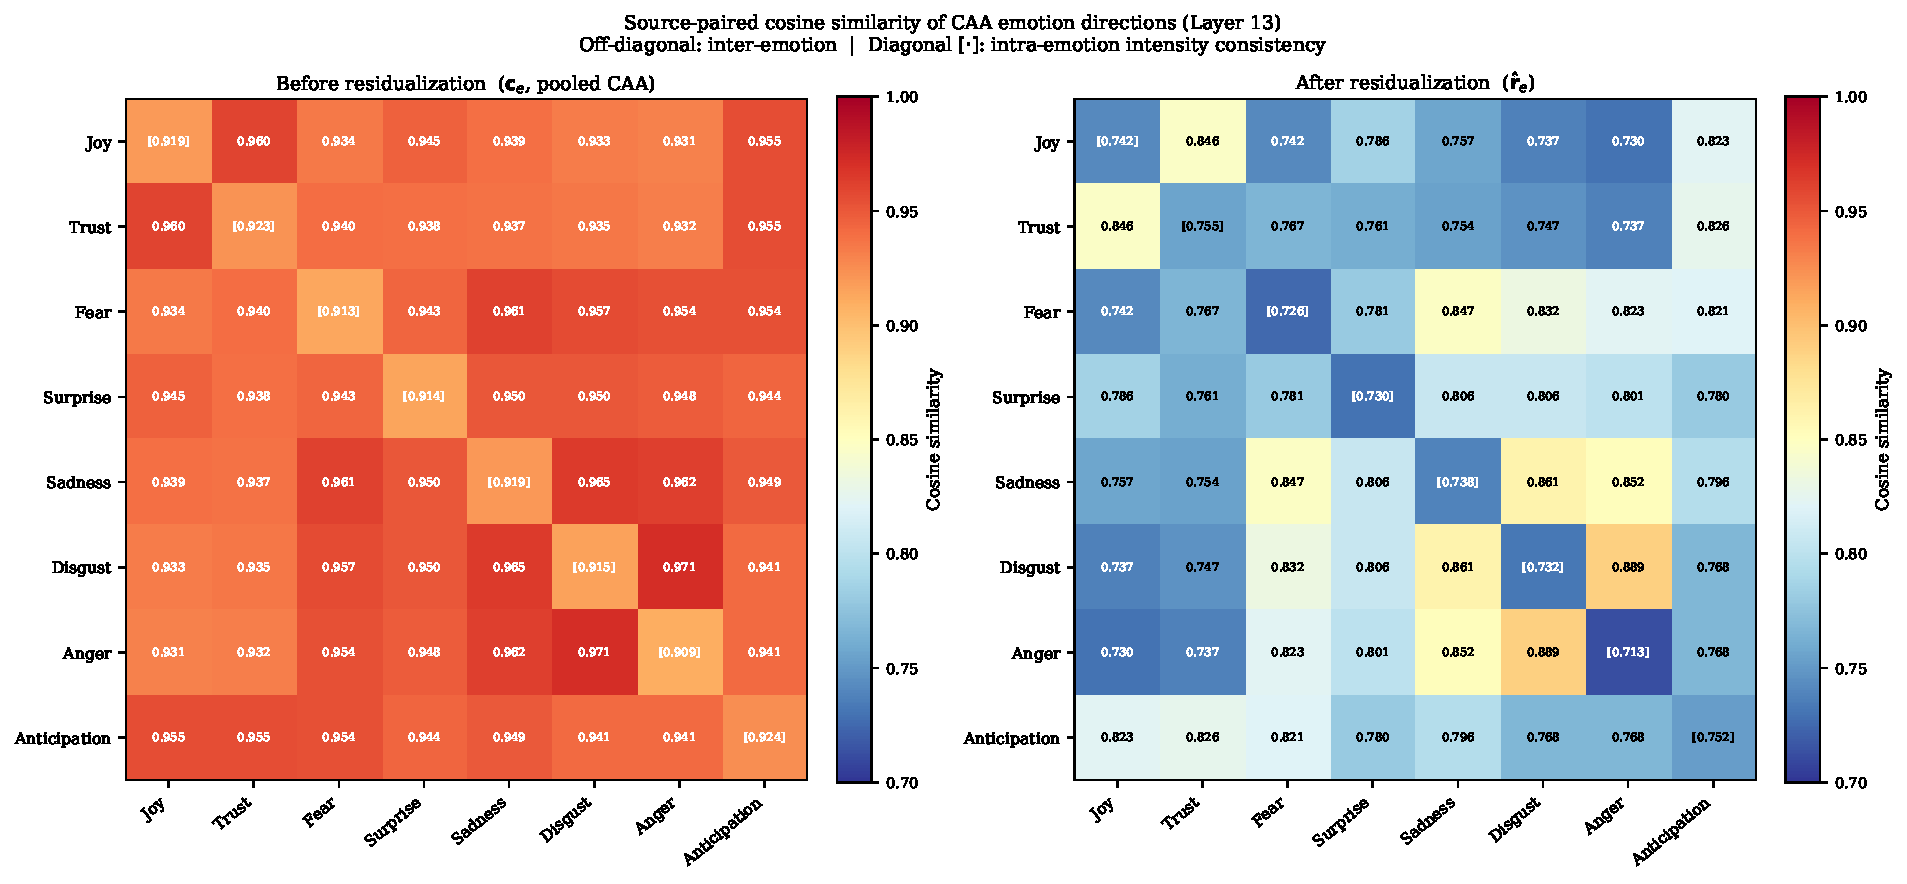
\includegraphics[width=\linewidth]{figures/caa_decomposition_cosine_before_after_L13.pdf}
    \caption{層13における$\mathbf{g}$の残差化前（左、$\mathbf{c}^{\mathrm{pool}}_e$）と後（右、$\hat{\mathbf{r}}_e$）の感情方向のソースペアコサイン類似度。非対角エントリは感情間類似度を表し、括弧内の対角エントリは感情内強度一貫性を表す。残差化により感情間整合性の平均が$0.947$から$0.794$に低下し、$\mathbf{g}$が感情横断的共線性の支配的な原因であったことが確認される。}
    \label{fig:caa_decomposition_cosine_before_after_L13}
\end{figure}

\subsection{線形プローブ精度}

$\hat{\mathbf{r}}_e$が感情アイデンティティを正確に捉えるならば、8クラス分類タスクで感情が線形分離可能であるはずである。ソース特異的コントラストシフト$\Delta_{n,e}$（強度にわたって平均）から目標感情を予測するロジスティック回帰分類器（L-BFGS、8クラス、80/20ソースベース分割）を訓練する。参照方向として$\mathbf{c}^{\mathrm{pool}}_e$または$\hat{\mathbf{r}}_e$のいずれかを使用する。ソースベースの分割により、テストセットには訓練中に見られなかった発話のみが含まれることが保証される。\par

結果を表~\ref{tab:linear_probe_accuracy}に示す。残差化前、プローブはチャンス率$12.5\%$に対して$92.7\%$の精度を達成する。残差化後、精度はわずかに$93.8\%$に増加する。精度の低下がないことは、$\mathbf{g}$が感情識別情報を持たないことを確認する。$\mathbf{g}$は全八つの感情にわたって共有されており、したがってそれらを区別することができない。わずかな改善は、$\mathbf{g}$を除去することで感情方向間の共線性が低減され、感情特異的信号が強化されることを示唆する。\par

\begin{table}[H]
\centering
\small
\begin{tabular}{lc}
\toprule
\textbf{条件} & \textbf{8クラス精度} \\
\midrule
チャンス & 12.5\% \\
残差化前（$\mathbf{c}^{\mathrm{pool}}_e$） & 92.7\% \\
残差化後（$\hat{\mathbf{r}}_e$） & \textbf{93.8\%} \\
\bottomrule
\end{tabular}
\caption{層13における8クラス感情分類の線形プローブ精度。精度はホールドアウトソース分割（80/20）で測定される。残差化後のわずかな改善は、$\mathbf{g}$が感情識別情報を含まないことを確認する。}
\label{tab:linear_probe_accuracy}
\end{table}

\subsection{プルチック円形構造}

第三の一貫性チェックは、残差方向がプルチックの感情の輪によって予測される隣接構造を反映するかどうかを検証する。この輪（図~\ref{fig:Plutchik}）では、八つの基本感情が円形に配置されている。隣接ペア（輪距離1、例：\textit{joy}--\textit{trust}）は対向ペア（輪距離4、例：\textit{joy}--\textit{sadness}）よりも密接に関連している。$\hat{\mathbf{r}}_e$が有効な感情表現であれば、そのコサイン類似度は輪距離が増加するにつれて単調に減少するはずである。\par

\begin{figure}[H]
    \centering
    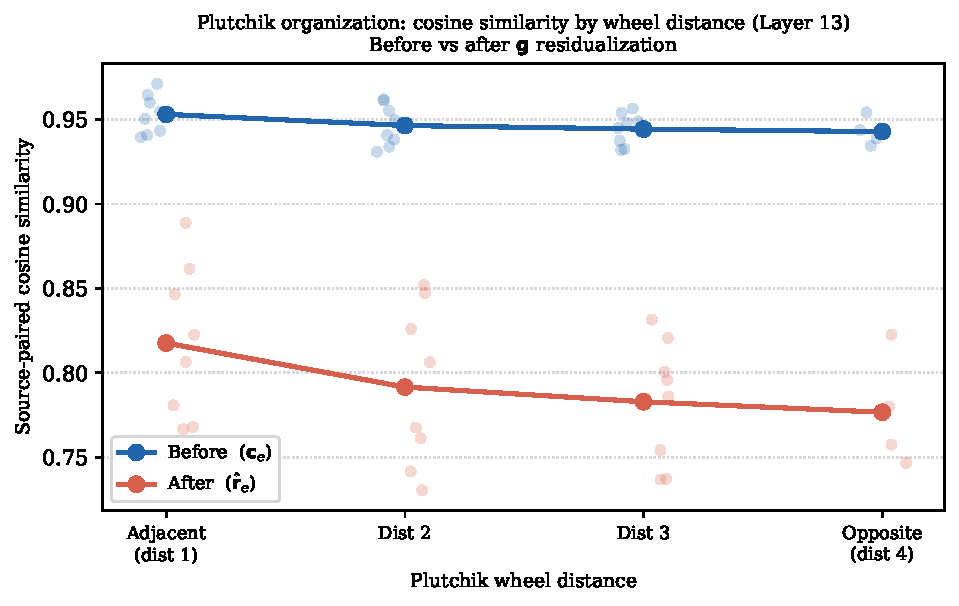
\includegraphics[width=0.65\linewidth]{figures/caa_decomposition_plutchik_L13.pdf}
    \caption{プルチックの輪距離（1=隣接、4=対向）でグループ化した平均ソースペアコサイン類似度。層13における$\mathbf{g}$の残差化前（青）と後（橙）。単調減少傾向は両条件で見られるが、隣接−対向ギャップは残差化後に$0.010$から$0.041$へと四倍に拡大する。}
    \label{fig:caa_decomposition_plutchik_L13}
\end{figure}

全28の感情ペアを輪距離（1〜4）でグループ化し、残差化前後で各グループ内の平均コサイン類似度を計算した。結果を図~\ref{fig:caa_decomposition_plutchik_L13}に示す。残差化前、単調傾向は可視だがほとんど知覚できない。隣接ペア（距離1、平均$= 0.953$）と対向ペア（距離4、平均$= 0.943$）の間のギャップはわずか$0.010$である。残差化後、このギャップは$0.041$に拡大し、四倍の増加となる。コサイン値は距離1の$0.818$から距離4の$0.777$へと明確に減少し、全四つのビンにわたってほぼ線形の勾配を示す。\par

表~\ref{tab:plutchik_pairs}は各ペアを詳細に調べる。隣接ペア\textit{Disgust}--\textit{Anger}が残差化後最高のコサイン（$0.889$）を達成し、直径対向ペア\textit{Trust}--\textit{Disgust}が最低値（$0.747$）を達成する。注目すべき例外は\textit{Fear}--\textit{Anger}である。これらは輪上で極対向にあるにもかかわらず、残差化後もコサインは$0.823$と高いままである。両感情は負の感情価と高覚醒を共有している。$\mathbf{g}$は全八つの感情に共通する平均方向として定義されるため、正/負の感情価軸はこの平均と一致せず、したがって$\hat{\mathbf{r}}_e$内に残る。これは一次元分解の既知の限界である。より完全な因子分解では、追加的な感情価軸が抽出されるだろう。しかし、\ref{sec:steering_causal_validation}節で示すように、この限界はコアステアリングパイプラインに測定可能な影響を与えない。\par

\begin{table}[H]
\centering
\small
\begin{tabular}{llcc}
\toprule
\textbf{ペア} & \textbf{タイプ} & \textbf{前} & \textbf{後} \\
\midrule
Disgust~--~Anger         & 隣接 & 0.971 & 0.889 \\
Sadness~--~Disgust       & 隣接 & 0.965 & 0.861 \\
Joy~--~Trust             & 隣接 & 0.960 & 0.846 \\
Anticipation~--~Joy      & 隣接 & 0.955 & 0.823 \\
\midrule
Fear~--~Anger            & 対向 & 0.954 & 0.823 \\
Surprise~--~Anticipation & 対向 & 0.944 & 0.780 \\
Joy~--~Sadness           & 対向 & 0.939 & 0.757 \\
Trust~--~Disgust         & 対向 & 0.935 & 0.747 \\
\bottomrule
\end{tabular}
\caption{プルチックの輪上の選択された隣接ペアおよび対向ペアに対する残差化前後のソースペアコサイン類似度。\textit{fear}--\textit{anger}の対向ペアは、平均方向残差化では除去されない共有の負感情価・高覚醒特性により、残差化後も高いまま（$0.823$）である。}
\label{tab:plutchik_pairs}
\end{table}

\subsection{まとめ}

三つの証拠ラインが全て同一の結論に収束する。$\mathbf{g}$と$\hat{\mathbf{r}}_e$への分解は幾何学的に妥当である。表~\ref{tab:decomposition_validity_summary}に主要な数値を収集する。共有成分$\mathbf{g}$は生のCAAベクトルにおける高い感情間整合性の原因である。それを除去すると、より識別力があり、完全な感情カテゴリ情報を保持し、プルチックの輪の理論的円形構造をより良く反映する残差が残る。一つの残差的限界、すなわち\textit{fear}--\textit{anger}コサインの上昇は、三つの全テストにわたって一貫している。これは分解自体の欠陥ではなく、$\mathbf{g}$のスパン外に存在する感情価軸を指している。\par

\begin{table}[H]
\centering
\small
\begin{tabular}{lcc}
\toprule
\textbf{テスト} & \textbf{前（$\mathbf{c}^{\mathrm{pool}}_e$）} & \textbf{後（$\hat{\mathbf{r}}_e$）} \\
\midrule
感情間コサイン（非対角平均） & 0.947 & 0.794 \\
8クラスプローブ精度          & 92.7\% & \textbf{93.8\%} \\
プルチック隣接−対向ギャップ  & 0.010 & \textbf{0.041} \\
\bottomrule
\end{tabular}
\caption{層13における分解妥当性テストのまとめ。矢印は有効な分解の下で期待される方向を示す。感情間コサインは減少すべき（感情方向がより独立になる）、プローブ精度は維持または改善すべき（感情情報が保持される）、そしてプルチックギャップは増加すべき（円形構造がより可視化される）である。}
\label{tab:decomposition_validity_summary}
\end{table}

\section{ステアリング介入のパラメータスイープ}
\label{sec:steering_experiments}

感情特異的残差$\hat{\mathbf{r}}_e$が目標感情に向けてテキスト生成を因果的に偏向させるかどうか、およびいかなるスケールでも共有ベクトル$\mathbf{g}$を組み込むことでさらなる恩恵が得られるかどうかを調査する。感情書き換えデータセットのテスト分割からサンプリングした100件のソース発話を用いて、\texttt{Llama-3.1-8B-Instruct}でフォローアップ文を生成する。交絡因子としてのサンプリング分散を排除するため、全体を通じて貪欲復号（温度$= 0$）を使用する。

\subsection{活性化フック}
\label{subsec:activation_hook}
ステアリング介入はトランスフォーマーの層13に登録されたフォワードフックとして実装される。各順伝播において、フックは残差ストリームの隠れ状態$\mathbf{h} \in \mathbb{R}^{B \times T \times D}$を捕捉し、最終トークンスライスのみに$\Delta_e$を加算する：
\[
\mathbf{h}_{:,\,-1,\,:} \;\leftarrow\; \mathbf{h}_{:,\,-1,\,:} + \Delta_e(\alpha_G, \alpha_R),
\]
ここで$\Delta_e = \alpha_G\,\mathbf{g} + \alpha_R\,\hat{\mathbf{r}}_e$である。摂動を最終プロンプトトークンのみに適用することで、自己回帰生成が開始する時点に因果信号を集中させ、先行する全トークンのコンテキスト表現を変更しないままにする。フックは生成完了直後に解放され、呼び出し間の干渉を防ぐ。

\subsection{スイープ設計}

二つの相補的なスイープを実施する。

\begin{enumerate}
  \item \textbf{$\alpha_R$スイープ} \\
  $\alpha_G = 0$を固定（残差成分を分離するため）し、$\alpha_R$を17個の等間隔値$\{-128,\,-112,\,-96,\,-80,\,-64,\,-48,\,-32,\\\,-16,\,0,\,16,\,32,\,48,\,64,\,80,\,96,\,112,\,128\}$でスキャンする。アンカー$\alpha_R = 0$はステアリングなしのベースラインを再現する。負の値は目標感情から遠ざかる。大きな正の値は、生成テキストが劣化する一貫性の閾値に近づくか超えることが予想される。ソーステキスト、目標感情、$\alpha_R$値の各組み合わせが単一の生成を構成し、$100 \times 8 \times 17 = 13{,}600$件の生成テキストが得られる。
  \item \textbf{$\alpha_G$スイープ} \\
  上記の$\alpha_R$探索に基づき、$\alpha_R = 64.0$を固定し、$\alpha_G \in \{0, 2.0, 4.0, 8.0\}$をスキャンする。アンカー条件$\alpha_G = 0$は共有成分なしの純粋な残差ステアリングに対応する。中間値（$2.0$と$4.0$）は、スケールが有害になる前に$\mathbf{g}$からの小さな寄与が有益かどうかを検証する。同じ100件のテスト分割ソースと8つの目標感情を使用し、$100 \times 8 \times 4 = 3{,}200$件の生成テキストが得られる。
\end{enumerate}

\subsection{自動評価プロトコル}

各生成文は\texttt{gpt-4o-mini}が審判として採点する。全アイテムにわたって一貫した評価基準を保証するため、審判は採点範囲全体をカバーする三つの固定フューショット例を提示される：

\begin{itemize}
  \item 高品質な目標に一致する例
  \item 意味は保存されているが表現される感情が誤っている例
  \item 目標感情が部分的に存在するが命題的内容が目標外れの例
\end{itemize}

これらの例はテストアイテムを審判が見る前に評価スケールを固定する。スコアはOpenAIの構造化出力APIを厳格なJSONスキーマを使用して取得され、自由形式の解析を排除し、数値スコアと支配的感情ラベルが一貫した機械可読形式で返されることを保証する。評価者は介入条件（$\alpha_G$または$\alpha_R$）を知らされない。\par

$\alpha_R$スイープについては、アイテムごとに以下の三つの連続$[0,1]$指標を収集する：
\begin{itemize}
  \item \textbf{文の健全性}：生成された書き換えが一貫していて文法的に正しく、繰り返しがないかどうか。これは、他の指標の解釈を混乱させる可能性のある非一貫または変性した出力にフラグを立てる品質チェックとして機能する。
  \item \textbf{意味保存}：ソース発話のコア命題的内容が保持されているかどうか。審判は生成テキストを元のテキストと比較し、同じ出来事、エンティティ、関係が存在するかどうかを評価する。
  \item \textbf{目標感情強度}：出力が目標感情をどれだけ強く伝えるか。審判は目標感情ラベルを示され、生成テキストにおけるその感情の強度を、それが主要な感情かどうかに関わらず評価するよう求められる。
\end{itemize}

$\alpha_G$スイープについては、代わりに以下の指標を収集する：

\begin{itemize}
  \item \textbf{目標感情一致}：出力の主要な感情トーンが目標感情と一致するかどうか。審判は目標感情ラベルを示され、生成テキストがその感情を主要な感情として伝える度合いを評価するよう求められる。
  \item \textbf{意味保存}：ソース発話のコア命題的内容が保持されているかどうか。審判は生成テキストを元のテキストと比較し、同じ出来事、エンティティ、関係が存在するかどうかを評価する。
  \item \textbf{感情性}：出力が何らかの感情表現を含むかどうか。低いスコアは平坦で非一貫、または情動的に空虚な出力にフラグを立てる。これは品質チェックとして機能する。非一貫なテキストを生成することで目標感情一致が改善されるように見える介入は、この指標の対応する低下によって露呈される。
\end{itemize}

評価に使用する実際のシステムプロンプトは付録~\ref{app:eval_prompts}に示す。

\subsection{スイープ結果}
\label{sec:alpha_r_sweep}

\subsubsection*{$\alpha_R$スイープ結果}

\begin{figure}[H]
\centering
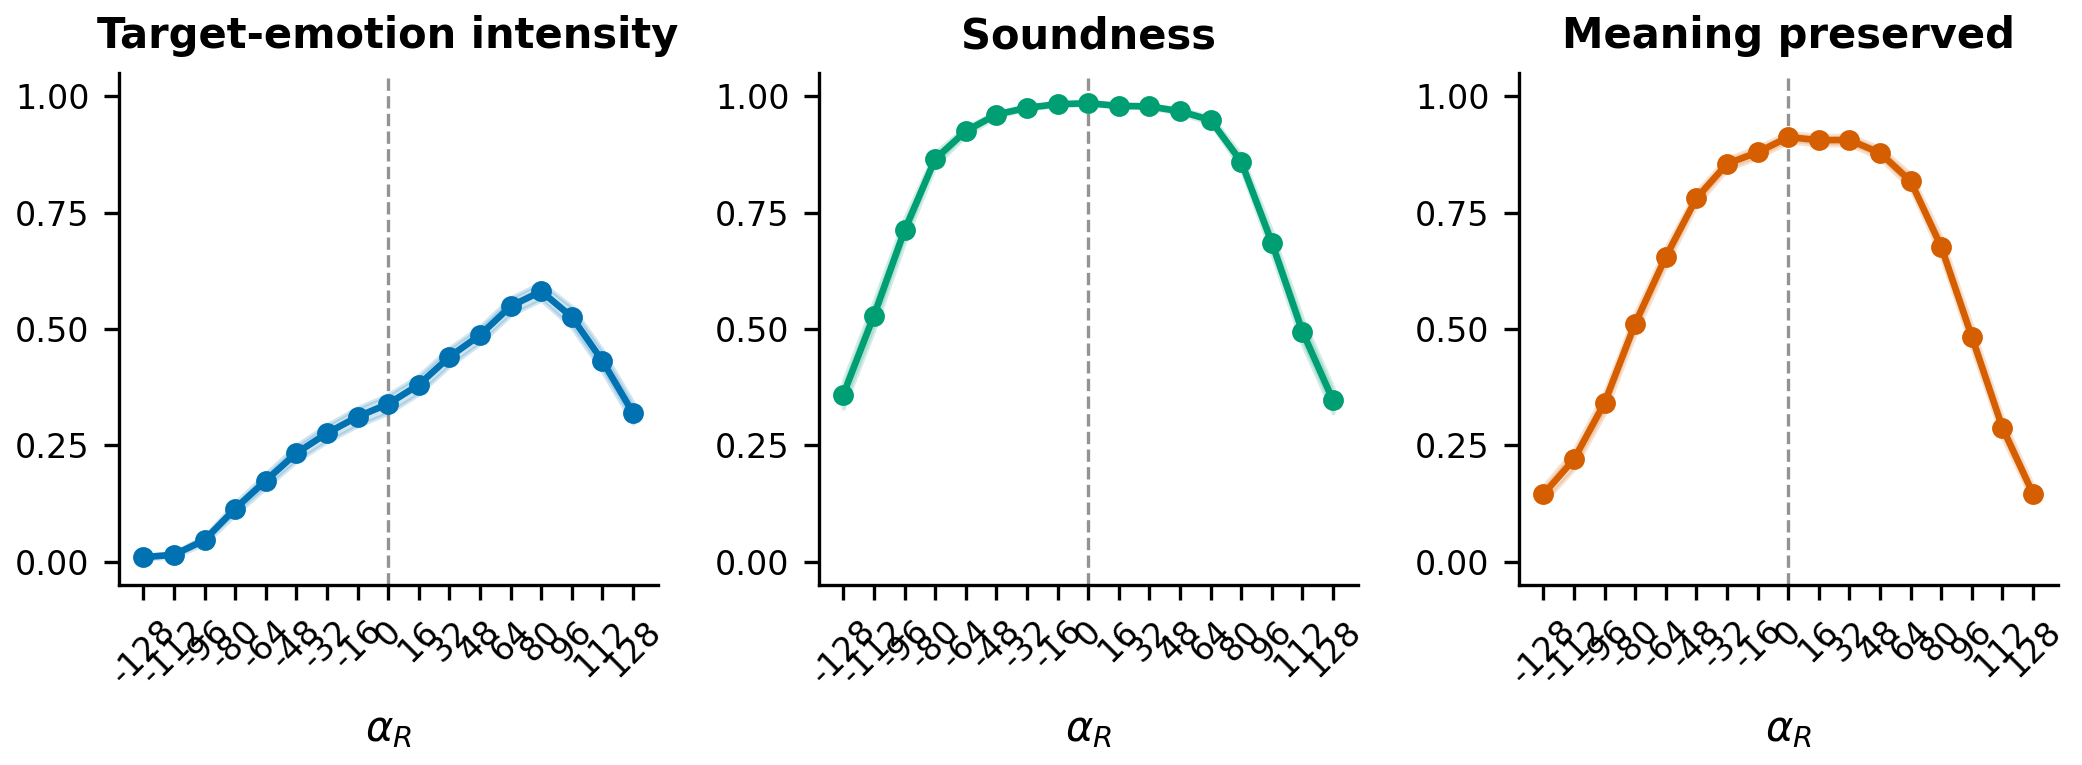
\includegraphics[width=\linewidth]{figures/alpha_r_sweep_fig1_aggregate_metrics.png}
\caption{$\alpha_R$の関数としての集計健全性、意味保存、目標感情強度（$\alpha_G = 0$固定；$n = 800$/条件；エラーバー = 95\% CI）。目標感情強度は$\alpha_R = 80$付近でピークを迎え、一貫性が劣化するにつれて低下する。健全性は$[-96, 80]$の外で急激に低下する。}
\label{fig:alpha_r_sweep_aggregate}
\end{figure}

図~\ref{fig:alpha_r_sweep_aggregate}は八つの感情にわたってプールされた三つの全指標を示す。健全性は$\alpha_R \in [-96,\, 80]$の間、$0.70$以上に維持される。この区間の外では、生成テキストは繰り返しや非一貫性へと劣化する。一貫した窓の中で、目標感情強度はステアリングなしのベースライン（$\alpha_R = 0$で$0.339 \pm 0.020$）から単調に増加し、$\alpha_R = 80$でピーク（$0.581 \pm 0.019$）に達し、$\alpha_R = 96$で一貫性が失敗するにつれて低下する。意味保存は健全性と密接に追随し、$\alpha_R = 0$の$0.912$から$\alpha_R = 80$の$0.677$へと低下し、より大きな摂動によるコンテンツ忠実度へのコストを反映する。\par

一貫した範囲に加えて、感情ごとに二つのサマリー指標を報告する。算術中点$M_A=(L_e+R_e)/2$は一貫した窓がステアリングなしのベースラインを中心に対称かどうかを測定する。ゼロに近い値は両方向で同様のヘッドルームがあることを示し、ゼロからの偏差は非対称なステアリング範囲を示す。また、$M_B$（一貫した範囲内で意味保存を最大化する$\alpha_R$の値）も報告する。これは生成テキストがソースの意味と最も近く整合する点を特定する。\par

\begin{table}[H]
\centering
\small
\begin{tabular}{lrrrrrr}
\toprule
\textbf{感情} & $L_e$ & $R_e$ & $M_A$ & $M_B$ & $\alpha_R^{+}$ & TI at $M_B$ \\
\midrule
anger        & $-112$ & $80$  & $-16$ & $48$ & $80$  & $0.570$ \\
anticipation & $-80$  & $128$ & $24$  & $0$  & $80$  & $0.567$ \\
disgust      & $-128$ & $80$  & $-24$ & $48$ & $80$  & $0.351$ \\
fear         & $-112$ & $96$  & $-8$  & $32$ & $80$  & $0.280$ \\
joy          & $-80$  & $96$  & $8$   & $0$  & $64$  & $0.472$ \\
sadness      & $-128$ & $128$ & $0$   & $0$  & $112$ & $0.249$ \\
surprise     & $-96$  & $64$  & $-16$ & $0$  & $32$  & $0.413$ \\
trust        & $-64$  & $96$  & $16$  & $0$  & $16$  & $0.536$ \\
\bottomrule
\end{tabular}
\caption{層13における感情ごとの一貫性閾値（$\alpha_G = 0$、健全性閾値$\geq 0.70$）。$L_e$/$R_e$：最左端/最右端の一貫した$\alpha_R$。$M_A$：一貫した範囲の算術中点。$M_B$：一貫した範囲内で意味保存を最大化する$\alpha_R$。$\alpha_R^{+}$：目標感情強度を最大化する$\alpha_R$（正側）。TI at $M_B$：$M_B$での目標感情強度。}\label{tab:alpha_r_thresholds}
\end{table}

表~\ref{tab:alpha_r_thresholds}と図~\ref{fig:alpha_r_sweep_thresholds}に示すように、一貫した範囲と最適動作点は感情によってかなり異なる。悲しみ（\textit{sadness}）が最も広い一貫した範囲（スイープ全体、$[-128, 128]$）を持ち、信頼（\textit{trust}）と驚き（\textit{surprise}）が最も制約されている（幅160）。\par

二つの感情が特に非対称なプロファイルを示す：\textit{anger}と\textit{disgust}である。両者について、一貫した範囲の中点はわずかに負（$M_A=-16$と$M_A=-24$）であり、意味保存が最高の点は正（$M_B=48$）である。したがって、$\alpha_R=0$はこれらのステアリング軸の自然な中心ではない。正の方向にわずかにシフトすることで元の意味がより良く保存され、これらの高覚醒・負感情価の残差がステアリングなし分布の中心に正確には位置しないことを示唆する。\par

$\alpha_R = 64$（全感情で一貫した範囲内にある）において、評価者は\textit{anger}ケースの90\%、\textit{joy}ケースの86\%で支配的な感情を正確に識別した。\textit{fear}と\textit{anticipation}の数値はそれぞれ78\%と66\%だった。\textit{disgust}（45\%）、\textit{sadness}（46\%）、特に\textit{surprise}（16\%）は頻繁に中性として分類され、これらの残差方向が評価者に強い感情として知覚されないスタイル的シフトを生成することを示している。\par

\begin{figure}[H]
\centering
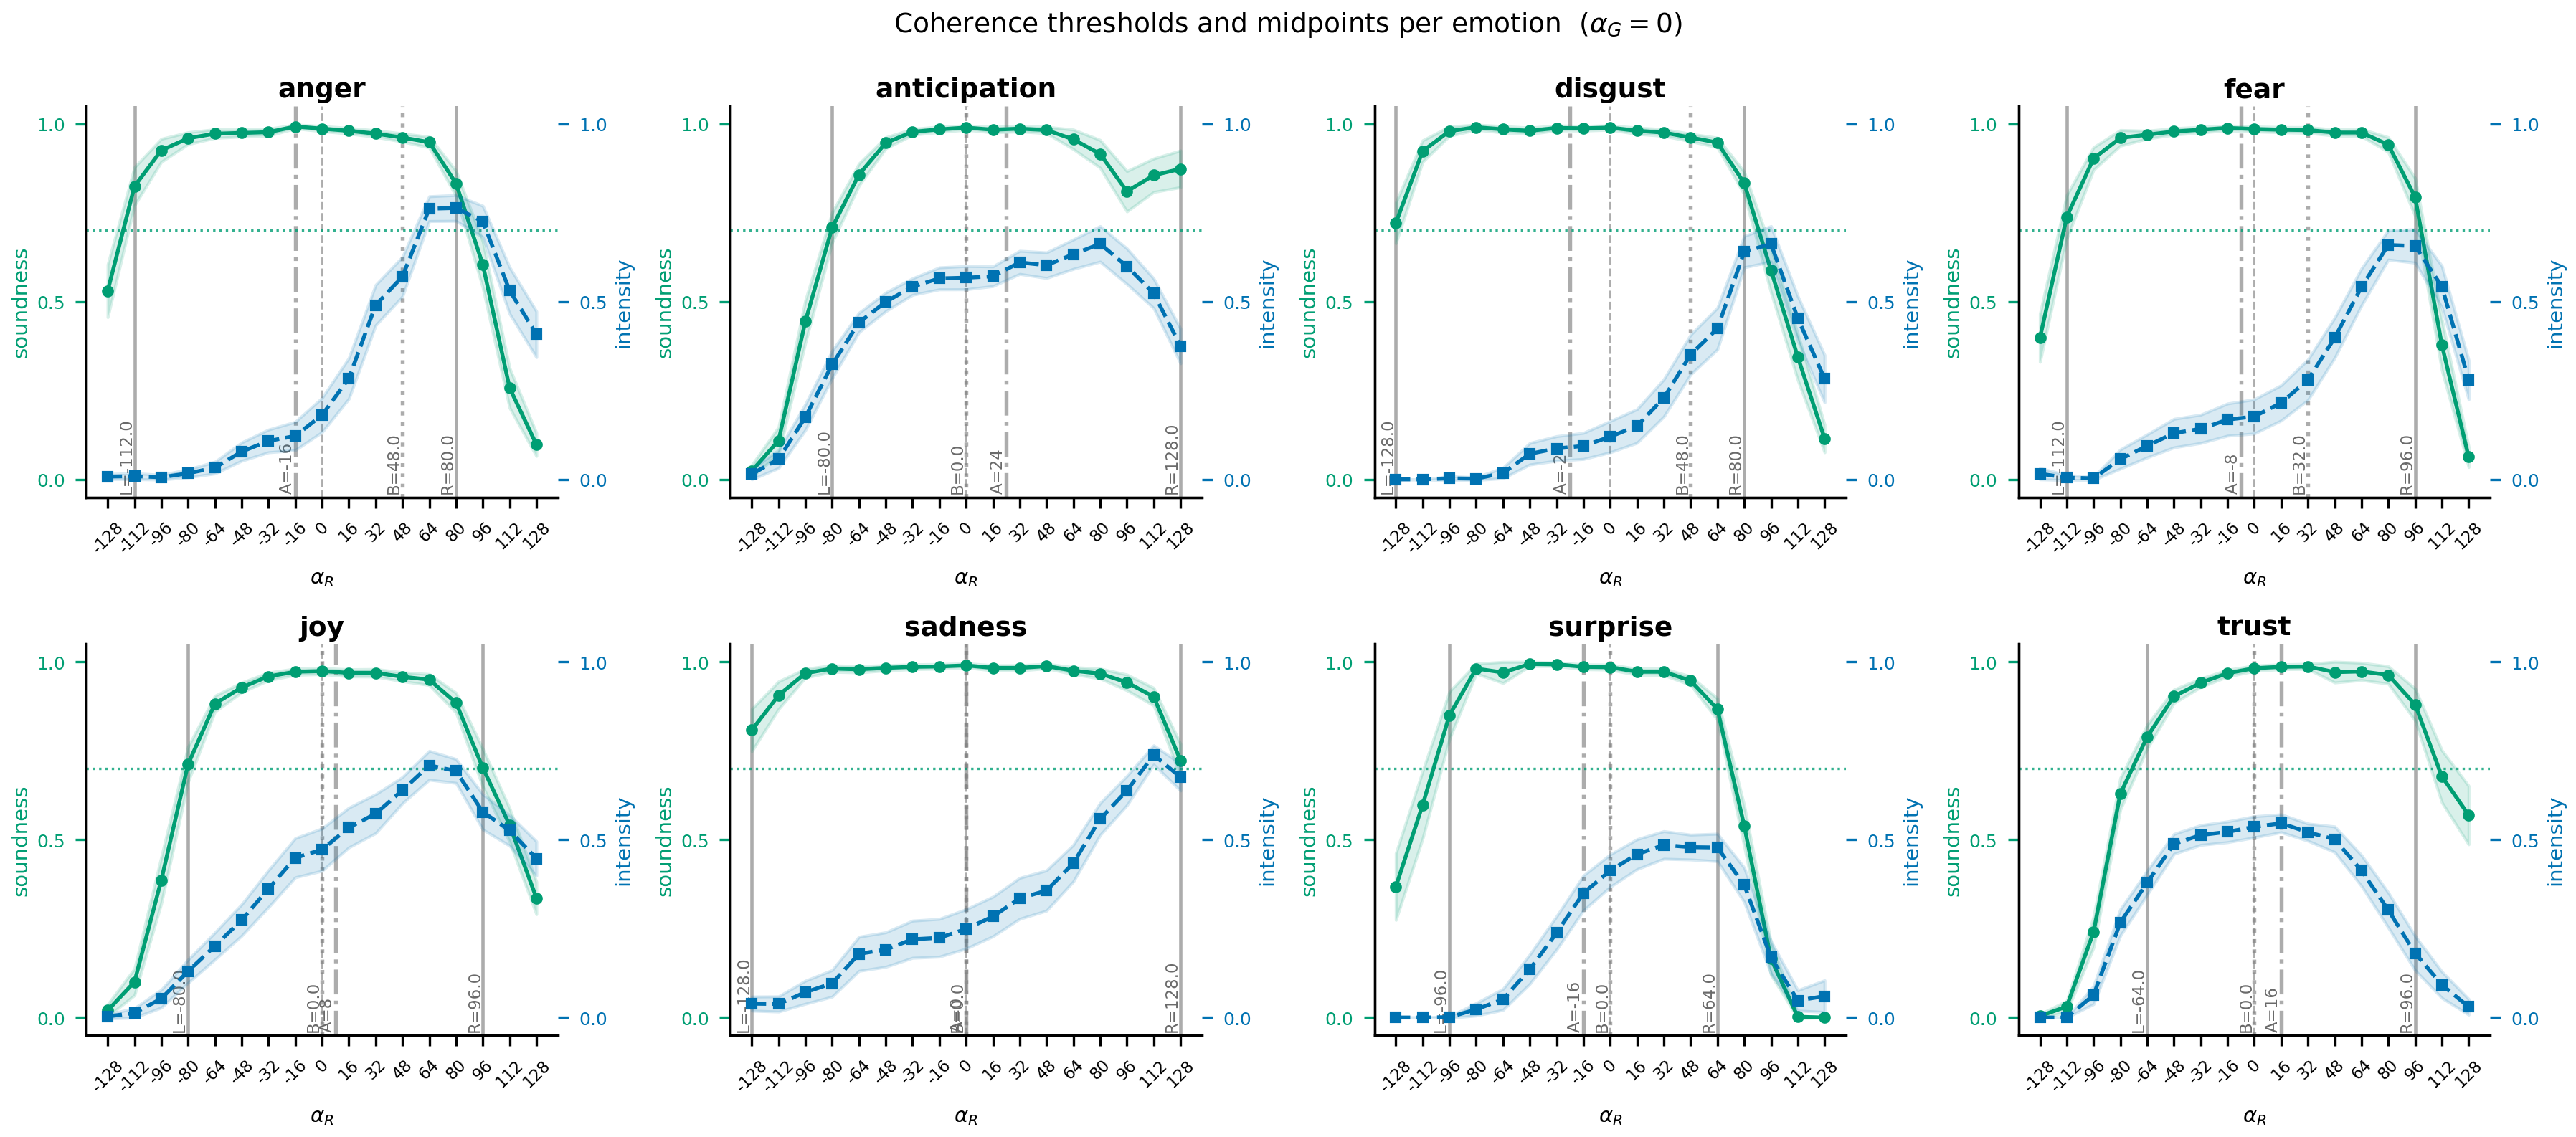
\includegraphics[width=0.9\linewidth]{figures/alpha_r_sweep_fig3_per_emotion_thresholds.png}
\caption{感情ごとの一貫性閾値。各サブプロットは健全性（緑、左軸）と目標感情強度（青、右軸）vs.\ $\alpha_R$を示す。垂直マーカー：$L_e$/$R_e$（最外端の一貫した$\alpha_R$）；$M_A = (L_e + R_e)/2$；$M_B$（一貫した範囲内で意味保存を最大化する$\alpha_R$）。}\label{fig:alpha_r_sweep_thresholds}
\end{figure}

\subsubsection*{異常分析}
信頼（\textit{trust}）は独特の応答パターンを示す。他の全感情とは異なり、その強度は$\alpha_R = 16$（$0.546$）でピークに達し、その後単調に減少し、$\alpha_R = 96$で$0.181$に達する。一貫した範囲内で最低の感情強度は最高の正の値、$\alpha_R = +96$で発生する。したがって、「信頼へ向けて」誘導することは逆説的に信頼の表現を抑制する。\par

一つの可能な説明は、\textit{trust}が指示チューニングとRLHF（人間フィードバックによる強化学習）によって誘導されたデフォルトのアシスタントペルソナと重複していることである。そのようなモデルはユーザの意図に従い、有益で好みに合った応答を生成するように訓練されており~\cite{bai2022traininghelpfulharmlessassistant,ouyang2022traininglanguagemodelsfollow}、信頼のような言語（例：安心感、従順さ、協力）はステアリングなしのベースラインですでに強い可能性がある。これは$\alpha_R = 0$での高いベースライン信頼強度$0.536$と一致している。\par

したがって、$\alpha_R$を増加させることでこのデフォルトレジスタをオーバーシュートし、モデルをより強い信頼として知覚されるよりも過度の安心感やおべっか・過度な追従的同意へと押し込む可能性がある。先行研究は、人間フィードバックで訓練されたモデルが、必ずしも真実または適切ではないがユーザの見解を好まれる方法で肯定するように学習できることを示している~\cite{wei2024simplesyntheticdatareduces,sharma2025understandingsycophancylanguagemodels}。より大きな正の$\alpha_R$での信頼強度の低下は、解釈可能な信頼から不自然なおべっかへのシフトを反映していると推測する。\par

\subsubsection*{負の$\alpha_R$と双極ステアリング}
$\alpha_R < 0$でのステアリングは$[L_e, 0]$内の一貫性を維持しながら目標感情を抑制する。四つの高覚醒・負感情価の感情（\textit{anger}、\textit{fear}、\textit{disgust}、\textit{surprise}）は、最も負の一貫した$\alpha_R$で健全性を$0.70$以上に維持しながら、ほぼゼロ（$\mathrm{TI} \approx 0.000$〜$0.006$）まで低減できる。正および社会的感情の抑制はより困難である：\textit{joy}は$\alpha_R = -80$で$\mathrm{TI} = 0.130$を維持し、\textit{anticipation}は同じ値で$0.323$を維持する。これらの知見は$\hat{\mathbf{r}}_e$の双極的解釈を支持するが、抑制の容易さは感情価カテゴリにわたって非対称である。

\subsubsection*{$\alpha_G$スイープ結果}
\label{sec:alpha_g_sweep}

\begin{figure}[H]
\centering
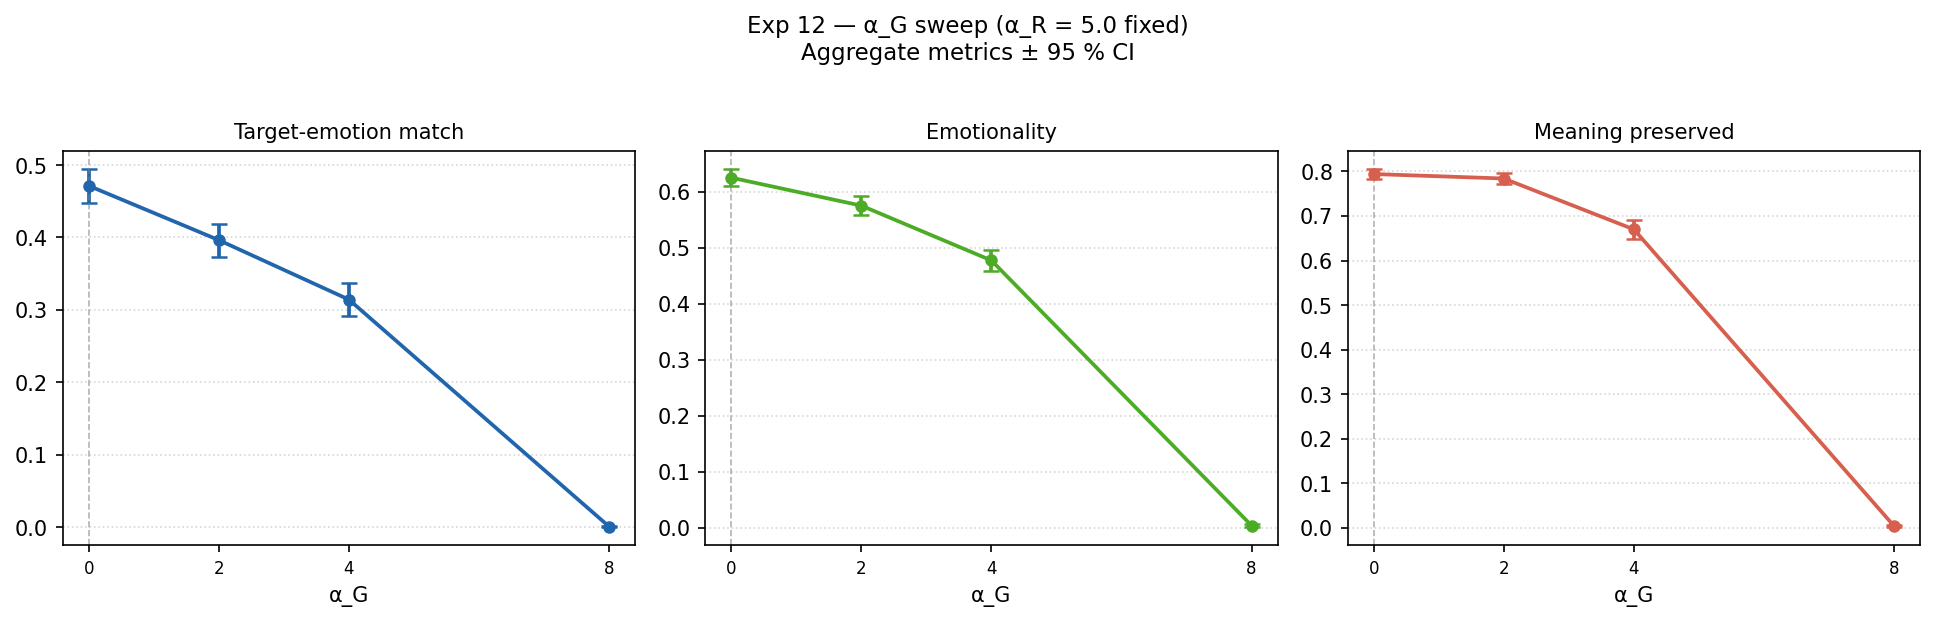
\includegraphics[width=\linewidth]{figures/alpha_g_sweep_aggregate.png}
\caption{$\alpha_G$の関数としての目標感情一致、感情性、意味保存（$\alpha_R = 64$固定；$n = 800$/条件；エラーバー = 95\% CI）。$\alpha_G$が$0$から増加するにつれて、三つの全指標が単調に減少する。}\label{fig:alpha_g_sweep_aggregate}
\end{figure}

\begin{figure}[H]
\centering
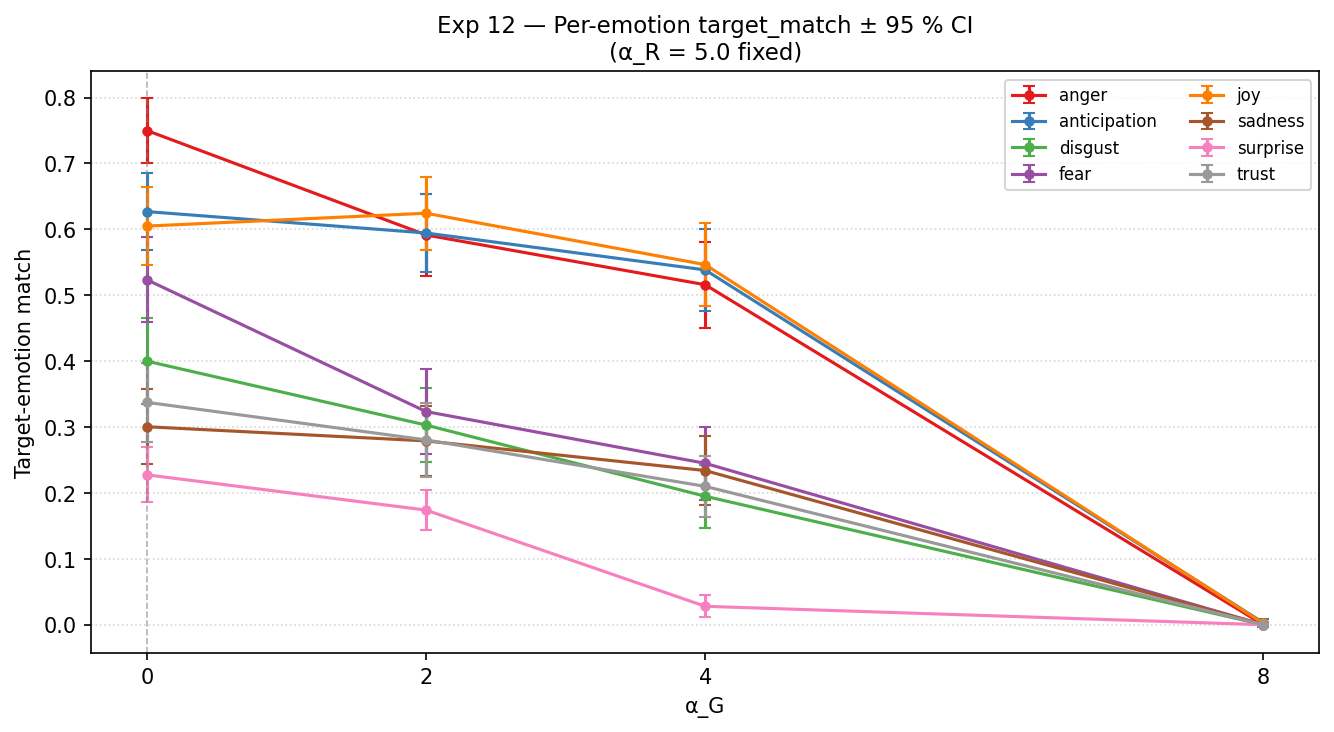
\includegraphics[width=0.7\linewidth]{figures/alpha_g_sweep_per_emotion.png}
\caption{感情ごとの目標感情一致 vs.\ $\alpha_G$（$\alpha_R = 64$固定；$n = 100$/セル；エラーバー = 95\% CI）。個々の感情は正の$\alpha_G$から恩恵を受けない。}\label{fig:alpha_g_sweep_per_emotion}
\end{figure}

$\alpha_R = 64.0$を固定し、$n = 800$サンプル/条件（$100$件のソーステキスト$\times$ $8$目標感情）にわたって$\alpha_G \in \{0, 2.0, 4.0, 8.0\}$をスイープする。これにより、$\mathbf{g}$を追加することがいかなるスケールでも有益かどうかを直接回答する。

図~\ref{fig:alpha_g_sweep_aggregate}は$\alpha_G$の関数として三つの全指標を示す。三つ全てが単調に低下する。目標感情一致は$\alpha_G = 0$の$0.471 \pm 0.023$から$\alpha_G = 2$の$0.396 \pm 0.023$、$\alpha_G = 4$の$0.314 \pm 0.023$へと低下し、$\alpha_G = 8$ではモデルが非一貫または空の出力を生成するため実質的にゼロになる。意味保存は$\alpha_G \in [0, 4]$にわたって$0.794$から$0.670$へと低下し、感情性も同じパターンに従う（$0.625$から$0.477$）。対応$t$検定により、劣化は全テストスケールで統計的に信頼できることが確認される。$\alpha_G = 2$単独での低下は$\Delta = -0.075$（$t = -7.68$、$p = 1.55 \times 10^{-14}$、$n = 800$ペア）である。唯一の例外は\textit{joy}で、$\alpha_G = 2$でわずかな増加を示す（$+0.020$）。これは95\%信頼区間（$\pm 0.023$）内に収まり、統計的に有意ではない。$\alpha_G > 0$のいかなる値も、いかなる指標でも信頼できる改善をもたらさない。感情ごとの内訳（図~\ref{fig:alpha_g_sweep_per_emotion}）は、個々の感情がいかなるテストスケールでも正の$\alpha_G$から恩恵を受けないことを確認する。

共有方向$\mathbf{g}$は感情特異的残差を分離するための分析的成分として有用である。しかし、全テストスケールで加算的な生成時ステアリング成分として逆効果である。したがって、効果的な情動ステアリングは$\Delta_e = \alpha_R\,\hat{\mathbf{r}}_e$に還元され、$\alpha_G$は廃棄される。

\subsection{定性的結果}
\label{sec:steering_causal_validation}

表~\ref{tab:cross_sadness_anger}は、\textit{sadness}を表現する文が\textit{anger}へとステアリングされた代表的な定性的例を提示する。定量的スイープ結果と一致する三つのパターンが浮かび上がる。\par

第一に、$\alpha_R$を増加させると感情的語彙だけでなく文の評価的フレーミングも変化する。$\alpha_R=16$では、出力は悲しみと後悔に近いままである。$\alpha_R=64$では、同じ喪失が不正義として再フレーミングされる。\textit{what was taken from me}という表現を通じて、出来事は受動的な欠如ではなく苦情として感じられるようになる。したがって、\textit{anger}の残差は単に怒りの言葉を追加するだけでなく、喪失の因果解釈を変える。\par

第二に、負のステアリングは出力を反対の感情方向に向ける。$\alpha_R=-64$では、文はもはや不正義を強調しない。代わりに、\textit{bittersweet nostalgia}や\textit{what I have cherished}などの表現を通じて、喪失の感覚が懐かしい受容へと和らげられる。これは$\hat{\mathbf{r}}_e$が双極的な感情軸として機能するという解釈を支持する。正の値は目標感情を強化し、負の値はそれを抑制または否定する。

第三に、過度の介入は出力品質を劣化させる。$\alpha_R=128$では、出力が繰り返しになり意味的に不安定になり、スイープで観察された一貫性の低下と一致する。共有成分$\mathbf{g}$を追加すると同様の劣化が発生する。$\alpha_G=4$では文が不完全になる。また、$\alpha_G=8$では繰り返しに陥る。この定性的パターンは、$\mathbf{g}$が共有感情性と感情特異的残差を分離する分析的目的には有用なままでありながら、生成時の制御成分として逆効果であるという定量的知見を支持する。

\begin{table}[H]
\centering
\small
\begin{tabular}{p{0.15\linewidth} p{0.78\linewidth}}
\toprule
\textbf{条件} & \textbf{ステアリング出力} \\
\midrule
\multicolumn{2}{l}{\textit{Base:} The old photographs reminded me of everything I had lost and would never get back} \\
\midrule

\begin{tabular}[t]{@{}l@{}}
$\alpha_R=16$ \\
$\alpha_G=0$
\end{tabular}
&
The old photographs stared back at me, a haunting reminder of all the fragments of my past that I could never reclaim, the memories that had slipped through my fingers like sand in the wind, and the love that had been irreparably lost. \\

\midrule

\begin{tabular}[t]{@{}l@{}}
$\alpha_R=64$ \\
$\alpha_G=0$
\end{tabular}
&
The old photographs brought back the pain of everything I've lost and the injustice of never being able to turn back time and reclaim what's been taken from me. \\

\midrule

\begin{tabular}[t]{@{}l@{}}
$\alpha_R=128$ \\
$\alpha_G=0$
\end{tabular}
&
They're a constant reminder of everything you're supposed to have to pay for your existence, but you can't even get a moment's justice, but they're just a waste of your time, but they can't be erased\ldots \\

\midrule

\begin{tabular}[t]{@{}l@{}}
$\alpha_R=-64$ \\
$\alpha_G=0$
\end{tabular}
&
The old photographs brought a bittersweet sense of nostalgia, but also a gentle reminder of the things I've cherished and the memories that will forever remain, even if some of the people and moments themselves have slipped away. \\

\midrule

\begin{tabular}[t]{@{}l@{}}
$\alpha_R=64$ \\
$\alpha_G=4$
\end{tabular}
&
Those old photographs brought back every memory of all the things I've lost and will never be able\ldots \\

\midrule

\begin{tabular}[t]{@{}l@{}}
$\alpha_R=64$ \\
$\alpha_G=8$
\end{tabular}
&
Those those old photographs brought all the memories of all the things I used \\

\bottomrule
\end{tabular}
\caption{ベース文「The old photographs reminded me of everything I had lost and would never get back」を$\hat{\mathbf{r}}_\text{anger}$でステアリングした結果。}
\label{tab:cross_sadness_anger}
\end{table}

\subsection{解釈}

スイープ結果から二つの主要な結論を導くことができる。第一に、共有方向$\mathbf{g}$は分析には有用だが、生成中には適していない。$\mathbf{g}$は中性から感情への共通シフトを捉えるが、生成中に追加することで一貫して目標感情整合性、意味保存、感情性が低下する。したがって、効果的な制御は残差項のみに還元される：
\[
\Delta_e = \alpha_R \hat{\mathbf{r}}_e .
\]

第二に、残差方向は制御可能で感情依存の情動軸として機能する。$\alpha_R$を増加させることで一貫性の限界まで目標感情が強化され、負の$\alpha_R$はそれを抑制し、$\hat{\mathbf{r}}_e$の双極的解釈を支持する。実際には、$\alpha_R=64$は保守的で高一貫性の設定を提供し、$\alpha_R=80$はより大きな意味的コストでより強い感情強度を得られる。例外は示唆に富んでいる：\textit{trust}ははるかに小さな値でピークに達し（$\alpha_R=16$）、指示整合とRLHF（人間フィードバックによる強化学習）によって誘導されたデフォルトのアシスタントレジスタとの重複を示唆する。\textit{surprise}は一方で、最適設定でも増幅が困難なままである。\par

\section{限界と移行}

これらの結果は、感情ステアリングが分解された残差空間における介入として、$\alpha_G = 0$および$\alpha_R > 0$の有効な動作点で実装できることを確認する。共有方向$\mathbf{g}$は全ての調べた指標で逆効果である。感情特異的残差$\hat{\mathbf{r}}_e$のみが信頼できるステアリング信号を提供する。この結論は、二つの成分を分離して独立に検証することを可能にした分解から直接導かれる。\par

しかし、これらの結果は二つの限界も明らかにする。第一に、ステアリング効果は絶対的ではなく控えめである。目標感情整合性は一貫して改善するが、天井にはほど遠く、介入はソース発話の意味的・感情的内容によって制約される。第二に、効果の大きさは感情によって大きく異なり、$\hat{\mathbf{r}}_e$の識別力がカテゴリによって異なることを示唆する。これは次章で取り上げられる構造的問題である。\par

これらの限界が次章を動機付ける。これまで$\hat{\mathbf{r}}_e$は単一のエンティティとして扱われてきた。次章では、この残差が実際に何を表しているかを調べる。具体的には、喜び（\textit{joy}）、悲しみ（\textit{sadness}）、怒り（\textit{anger}）などの感情がアトミックなベクトルとして扱われるべきか、それともより微妙な前言語的情動次元に対応する局所的な副軸を含むかどうかを調べる。\par
